%% using_orthologue_prediction.tex
%% Author: Leighton Pritchard
%% Copyright: James Hutton Institute
%% A brief introduction to orthologues, and evaluation of their prediction

% SUBSECTION: Why orthologues?
\subsection{Using orthologue predictions}

% Which methods work best
\begin{frame}
  \frametitle{Functional adaptation in \textit{Pba}\footnote{\tiny{Toth \textit{et al}. (2006) \textit{Ann. Rev. Phytopath.} \textbf{44}:305-336 \href{http://dx.doi.org/10.1146/annurev.phyto.44.070505.143444}{doi:10.1146/annurev.phyto.44.070505.143444}}}}
  \begin{center}
      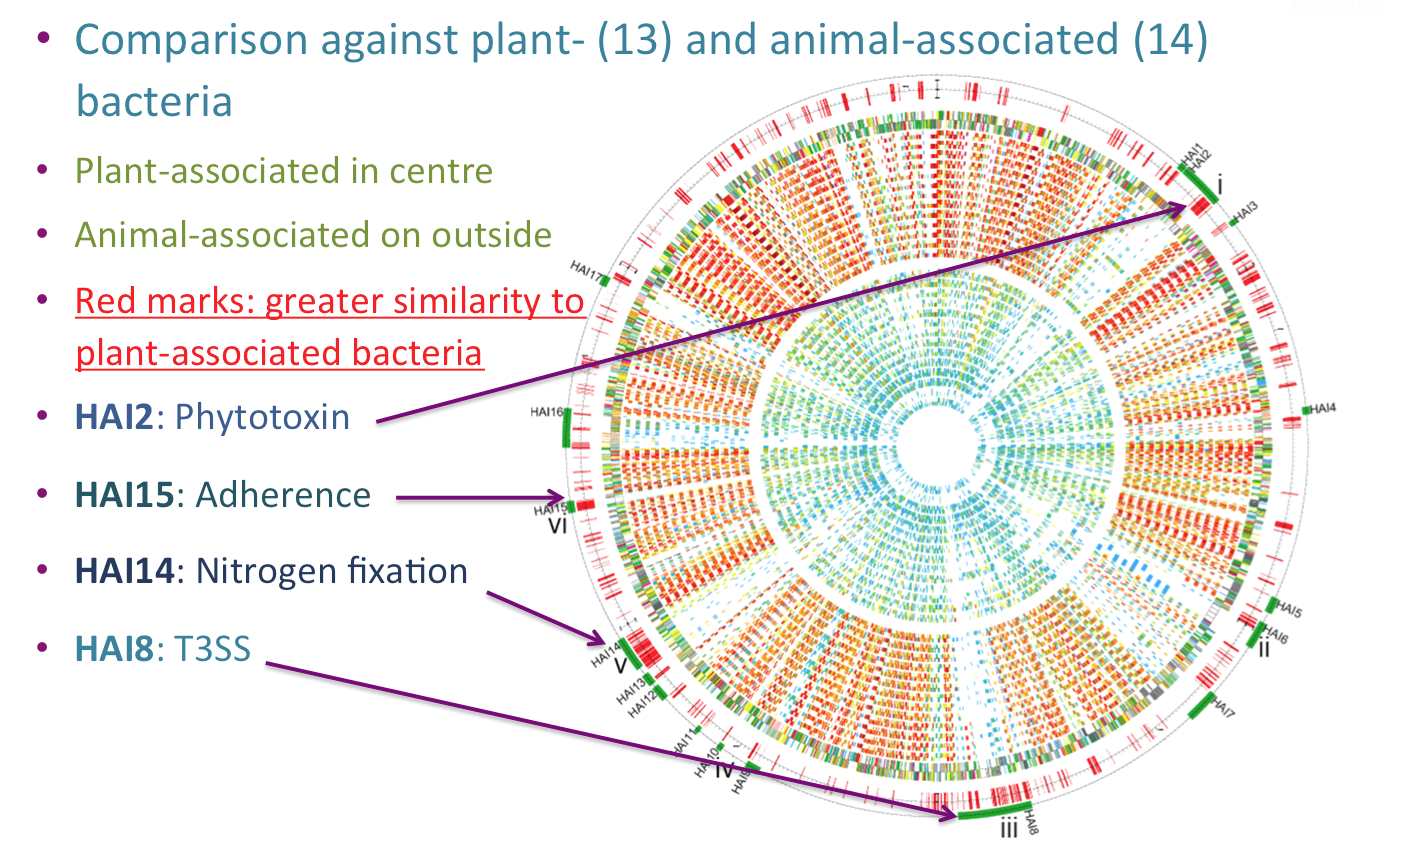
\includegraphics[width=1\textwidth]{images/pba_lgt} 
  \end{center}
\end{frame}

% Which methods work best
\begin{frame}
  \frametitle{Functional adaptation in \textit{Pba}\footnote{\tiny{Toth \textit{et al}. (2006) \textit{Ann. Rev. Phytopath.} \textbf{44}:305-336 \href{http://dx.doi.org/10.1146/annurev.phyto.44.070505.143444}{doi:10.1146/annurev.phyto.44.070505.143444}}}}
  \begin{center}
      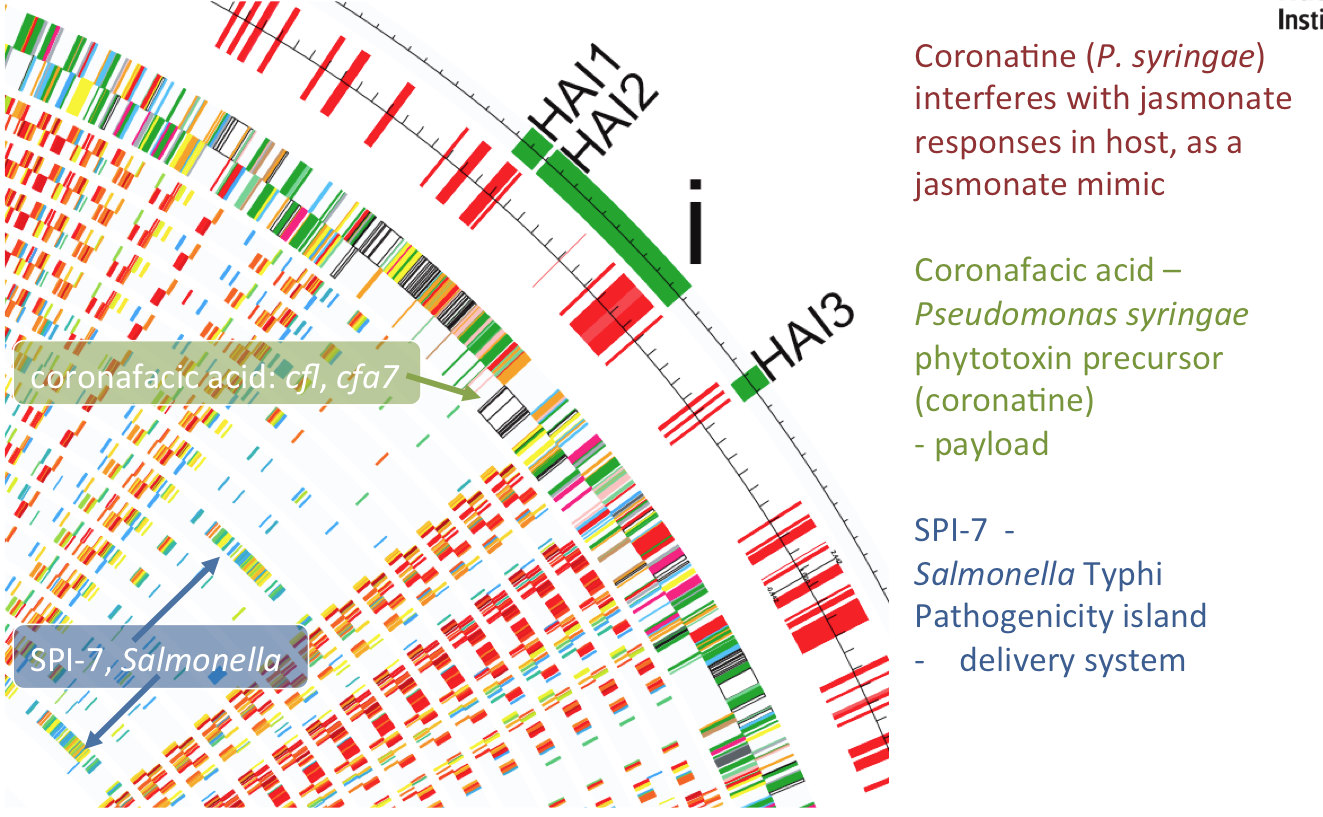
\includegraphics[width=1\textwidth]{images/pba_coronatine} 
  \end{center}
\end{frame}

% SUBSECTION: Core and pangenomes
\subsection{Core and Pan-genomes}

% Which methods work best
\begin{frame}
  \frametitle{Core genome}
  Once equivalent genes have been identified, those present in all related isolates can be identified: \textbf{\textit{the core genome}}.\\
  The \textit{core} genome is expected to underpin common function.\\
  A core RBH cluster (\textit{clique}) for 29 genomes:
  \begin{center}
      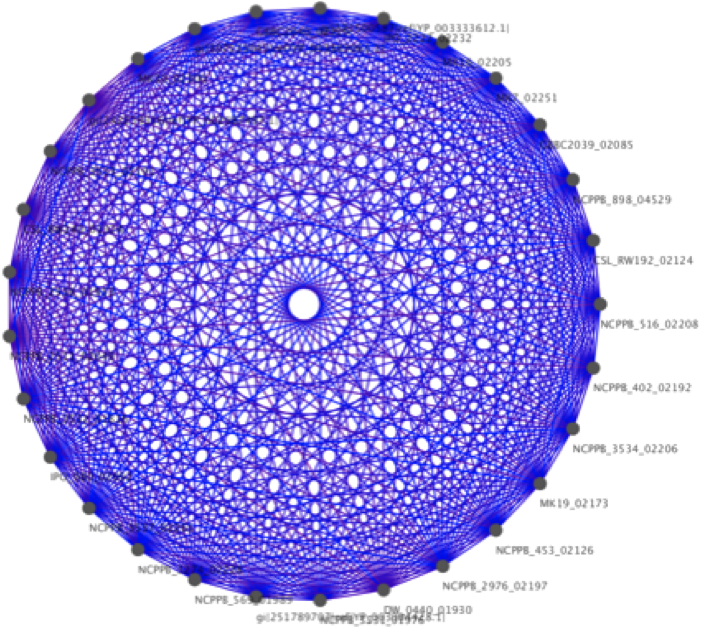
\includegraphics[height=0.55\textheight]{images/core_cluster} 
  \end{center}
\end{frame}

% Which methods work best
\begin{frame}
  \frametitle{Accessory genome}
  The remaining genes are \textbf{\textit{the accessory genome}}, and are expected to mediate function that distinguishes between isolates.\\[0.2cm]
  An accessory RBH cluster for 29 genomes:
  \begin{center}
      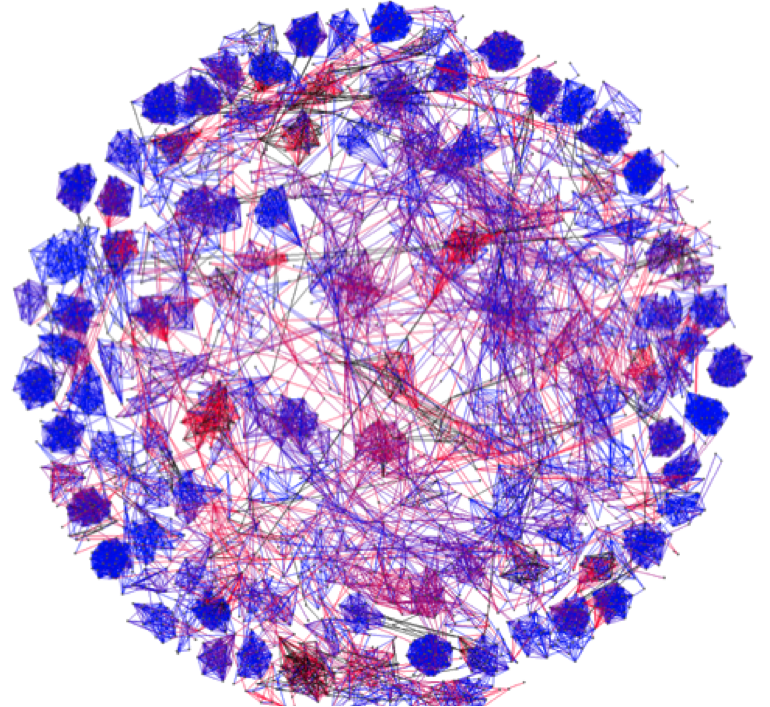
\includegraphics[height=0.5\textheight]{images/accessory_cluster} 
  \end{center}
\end{frame}

% Which methods work best
\begin{frame}
  \frametitle{Accessory clusters}
  Accessory RBH clusters can be pruned, to identify the accessory genome specific to subgroups of isolates:
  \begin{center}
      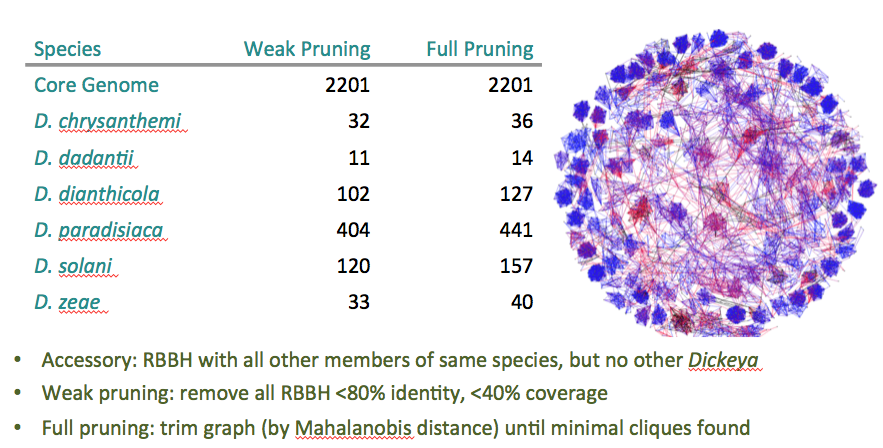
\includegraphics[height=0.55\textheight]{images/dickeya_accessory} 
  \end{center}
  These genes may be responsible for subgroup-specific phenotypes
\end{frame}

% Which methods work best
\begin{frame}
  \frametitle{Accessory genome
   \footnote{\tiny{Croll and Mcdonald (2012) \textit{PLoS Path.} \textbf{8}:e1002608 \href{http://dx.doi.org/10.1371/journal.ppat.1002608}{doi:10.1371/journal.ppat.1002608
  }}}
    \footnote{\tiny{Baltrus \textit{et al}. (2011) \textit{PLoS Path.} \textbf{7}:e1002132 \href{http://dx.doi.org/10.1371/journal.ppat.1002132.t002}{doi:10.1371/journal.ppat.1002132.t002
    }}}  
  }
  Accessory genomes act as a cradle for adaptive evolution \\[0.2cm]
  This is particularly so for bacterial pathogens, such as \textit{Pseudomonas} spp.
  \begin{center}
      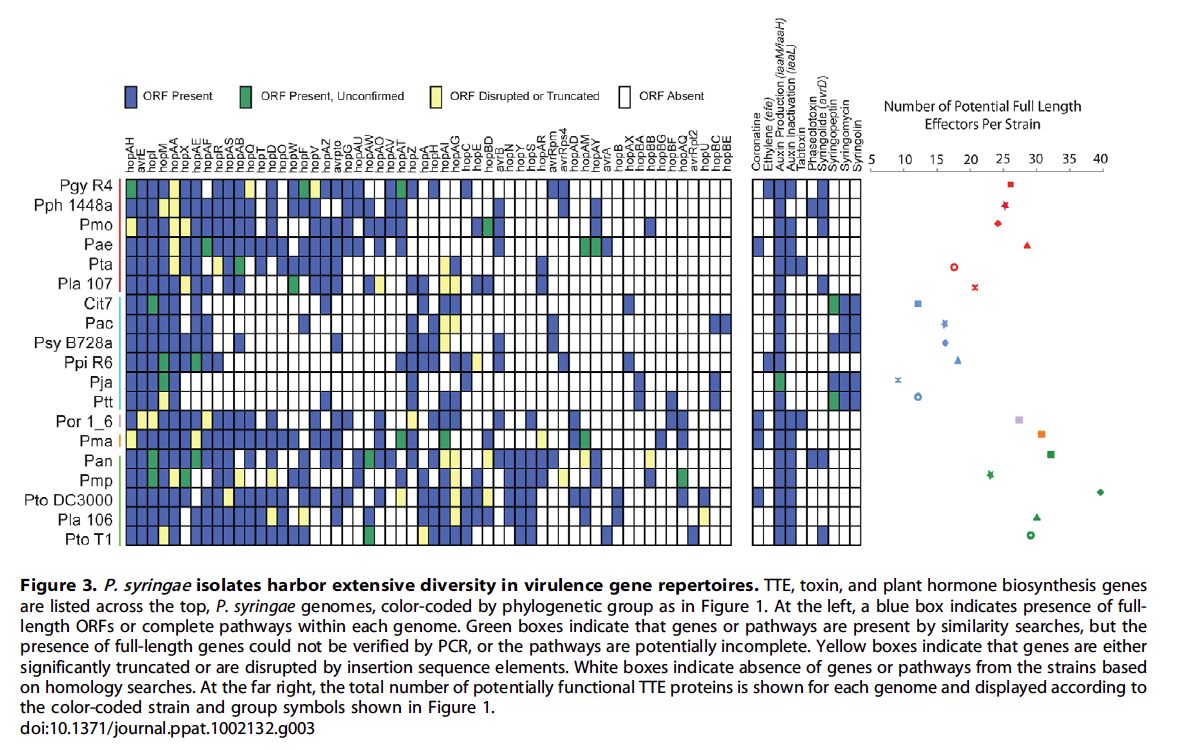
\includegraphics[height=0.5\textheight]{images/pa_virulence} 
  \end{center}
\end{frame}

% Which methods work best
\begin{frame}
  \frametitle{Core genome synteny
    \footnote{\tiny{Proost \textit{et al}. (2012) \textit{Nuc. Acids Res.} \textbf{40}:e11 \href{http://dx.doi.org/10.1093/nar/gkr955}{doi:10.1093/nar/gkr955
    }}}
  }
  Using tools like i-ADHoRe that identify synteny and collinearity, the structural organisation of the core genome can be determined:
  \begin{center}
      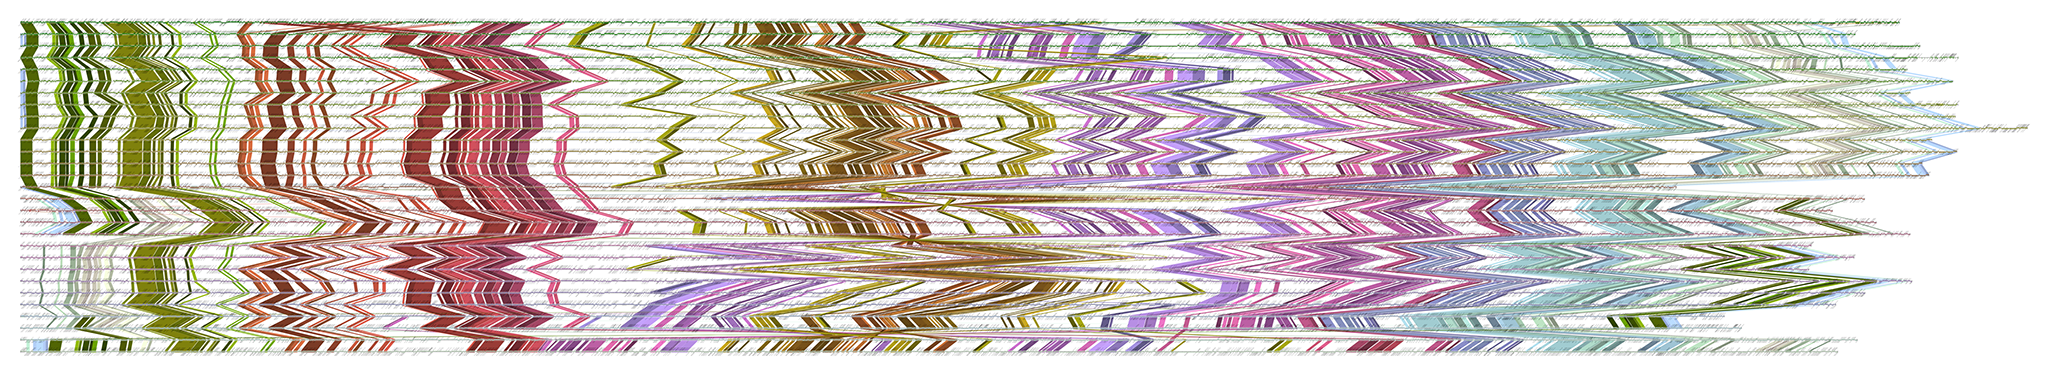
\includegraphics[width=1\textwidth]{images/dickeya_core_collinear_small} 
  \end{center}
  For \textit{Dickeya}, the core genome appears to be structurally well-conserved across all isolates.
\end{frame}

% Which methods work best
\begin{frame}
  \frametitle{Panseq\footnote{\tiny{Laing \textit{et al}. (2010) \textit{BMC Bioinf.} \textbf{11}:461 \href{http://dx.doi.org/10.1186/1471-2105-11-461}{doi:10.1186/1471-2105-11-461}}}}
  \texttt{Panseq} is an online tool for identification of core and accessory genomes, available at \href{https://lfz.corefacility.ca/panseq/}{https://lfz.corefacility.ca/panseq/}, and \href{https://github.com/chadlaing/Panseq}{https://github.com/chadlaing/Panseq} for standalone use
  \begin{center}
      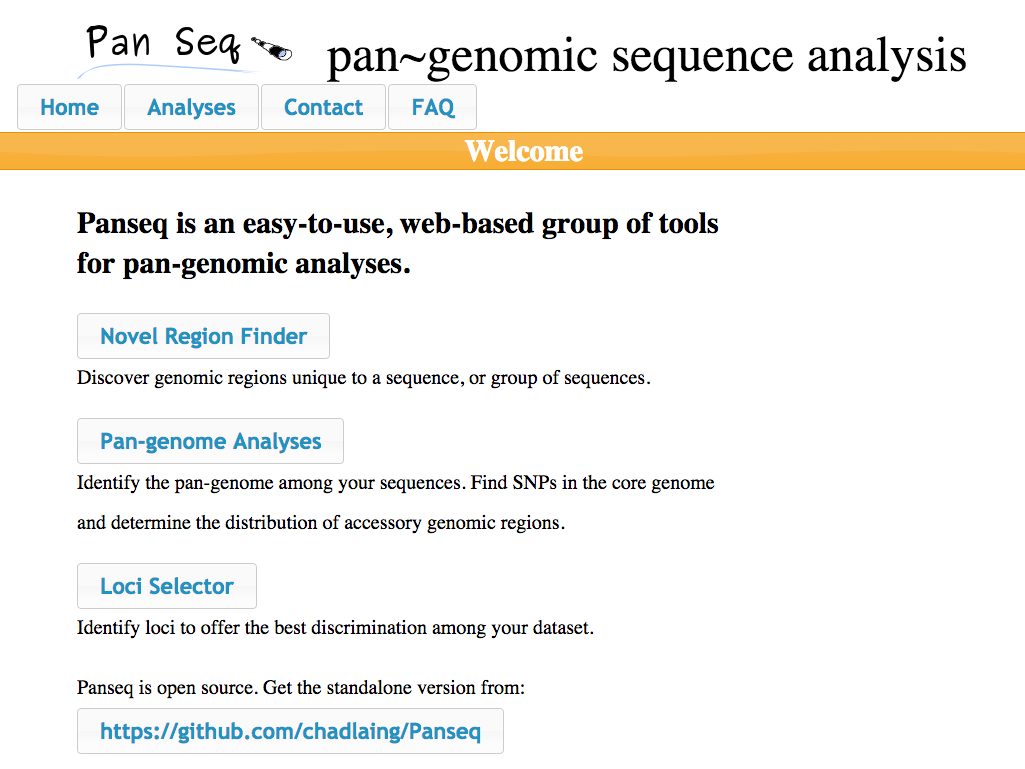
\includegraphics[width=0.7\textwidth]{images/panseq} 
  \end{center}
\end{frame}

%
\begin{frame}
  \frametitle{Harvest\footnote{\tiny{Treangen \textit{et al}. (2014) \textit{Genome Biol.} \textbf{15}:524 \href{http://dx.doi.org/10.1186/s13059-014-0524-x}{doi:10.1186/s13059-014-0524-x}}}}
  Visualising and organising comparison/pangenome data across thousands of bacteria is difficult.\\
  \textit{Very} recently (this week), the \texttt{Harvest} suite of tools was published, for alignment and visualisation of thousands of genomes:
  \begin{center}
      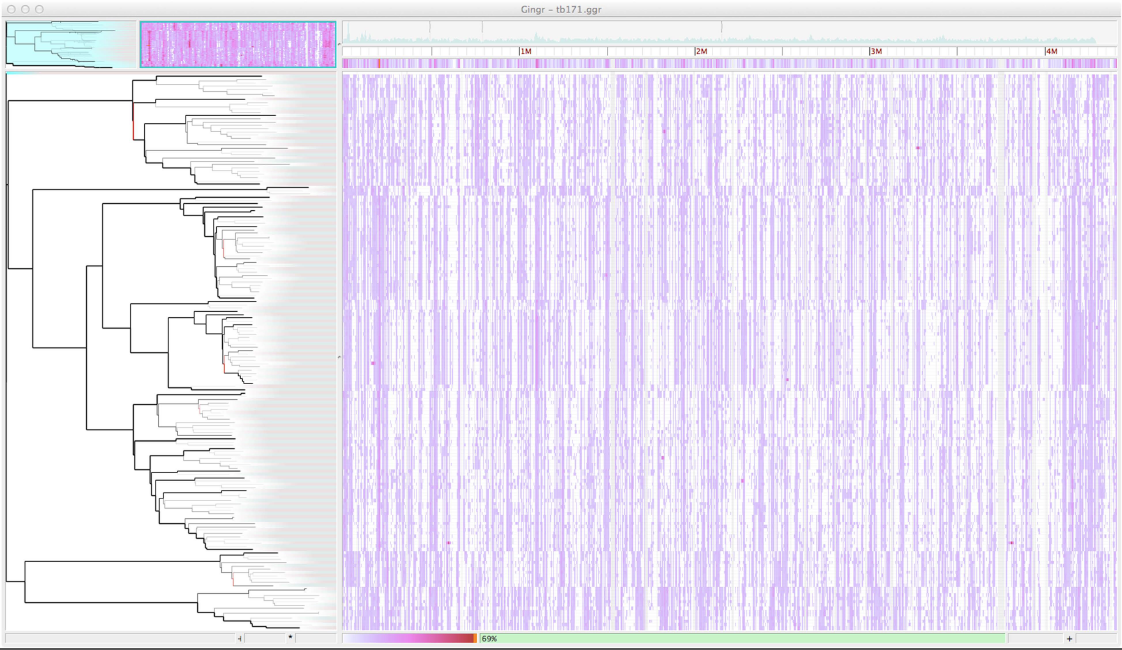
\includegraphics[width=0.8\textwidth]{images/harvest} 
  \end{center}
\end{frame}

